\documentclass{standalone}
\usepackage{standalone}

\begin{document}

\subsection{Gaussian Filter}
In this step, 2D Gaussian filter is applied to the gradient image from previous step. We used a Gaussian kernel of size $60 \times 60$. To calculate the kernel the formula in Equation \ref{eq:GaussFilter} is used. Figure \ref{fig:GaussianFilterPlot} shows a plot of this filter.
\begin{equation} \label{eq:GaussFilter}
g(i, j) = \dfrac{\alpha}{2\pi\sigma^2} \cdot e^{\frac{i^2 + j^2}{2\sigma^2}}
\end{equation}

\begin{figure} 
	\centering
	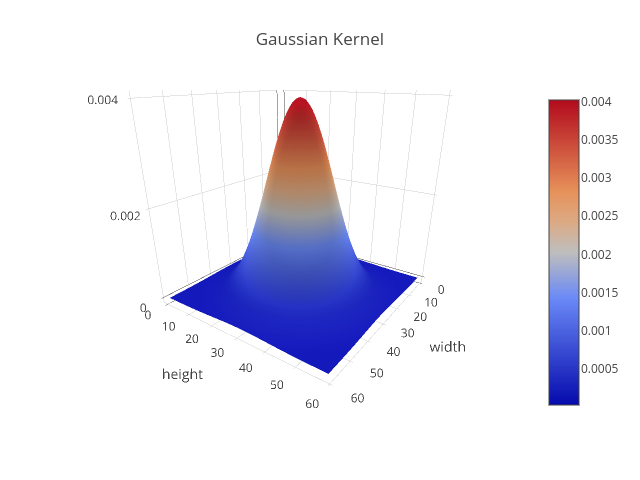
\includegraphics[width=.8\linewidth]{./img/plot/gauss.jpg}
	\caption{Applied the Gaussian Blur} 
	\label{fig:GaussianFilterPlot}
\end{figure}

Here, the blur coefficient $\alpha$ and the $\sigma$ are set empirically. We used $filter2D$ function to apply convolution of on the gradient image
\begin{lstlisting}[language=Python]
gauss = cv2.filter2D(sobel, cv2.CV_64F, kernel)
\end{lstlisting}

As a result we get a nicely blurred image (Figure \ref{fig:GaussianSample}).
\begin{figure} 
	\centering
	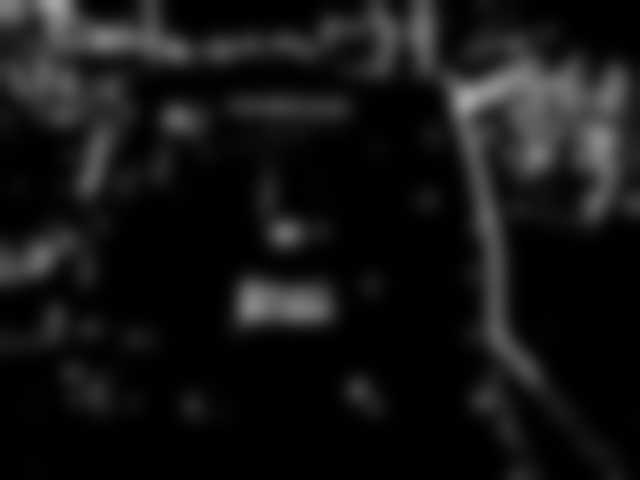
\includegraphics[width=.8\linewidth]{./img/sample/stage3.jpg}
	\caption{Applied the Gaussian Blur} 
	\label{fig:GaussianSample}
\end{figure}


\end{document}